%%
%% Template chap1.tex
%%

\chapter{EmpiricalStudy}

We carry out the empirical study between Stack Overflow and its corresponding Russian site in two perspectives, i.e., the users between them and the content within each site.

\section{Users}
In this part, we mainly analysis the whether it is necessary to build multilingual Stack Overflow by deeply compare the user activity, the knowledge base status and the areas of focus between Stack Overflow main site and Russian Stack Overflow site. The combination of all research results can lead to a solid conclusion for the meaning of multilingual Q\&A community development. \par 
It has been highly believed that the user is highly important for the analysis of a community because the whole knowledge base is the achievement of all users during a long time of accumulation. Users in the intersection of Stack Overflow main site user set and Russian Stack Overflow user set, who own both accounts should be considered as the main research object. According to the Stack Overflow policy, a user has a different user id on the specific site, while a unique account id, which is the way to link these two users on the entire Stack Exchange Network [4]. According to Table 1.1, By September 1st, 2017, there are 7,617,191 users on Stack Overflow main site and 86,826 users on Russian Stack Overflow site. We can easily get that there are 45,764 users owns both accounts at the same time, which is about 52.7\% of the total number of the user amount on Russian Stack Overflow.\par
\subsection{Creation Date}
Focusing on this intersection user base, the User Migration is calculated by comparing their account creation dates of each site. In this set, 16,155 users sign up their Russian Stack Overflow account first and then sign up for a Stack Overflow account, while the other 29,607 users are in a diametrical way. On one hand, the user base is segregated by the new sub-site and the number of users leaving the main site to their native language sub-site is growing with the time goes by. On the other hand, if we define a user migrate from one site to another by his or her account’s creation date, when 35 out of 100 users in the users who currently own both accounts migrate to Stack Overflow from Russian Stack Overflow, the other 65 of those 100 people migrate to Russian Stack Overflow from Stack Overflow, which means the Russian version offers a number of users as feedback to Stack Overflow main site. \par
To illustrate the user migration in details, Figure 2.1 presents the statics of the users who sign up a Russian Stack Overflow account from Jan 1st, 2014 to Sep. 1st, 2017. As we can see in the graph, the new users who migrated from Stack Overflow main site occupy a high proportion, and also the Russian site attracts and feedbacks a growing number of users to the main site with the time going by. In other words, the main site and the multilingual version both have a positive effect on the other one, which means both of them can assist the development of the other. This phenomenon means the development of multilingual version is helpful for the development of the main site.
\begin{figure}[!h]
	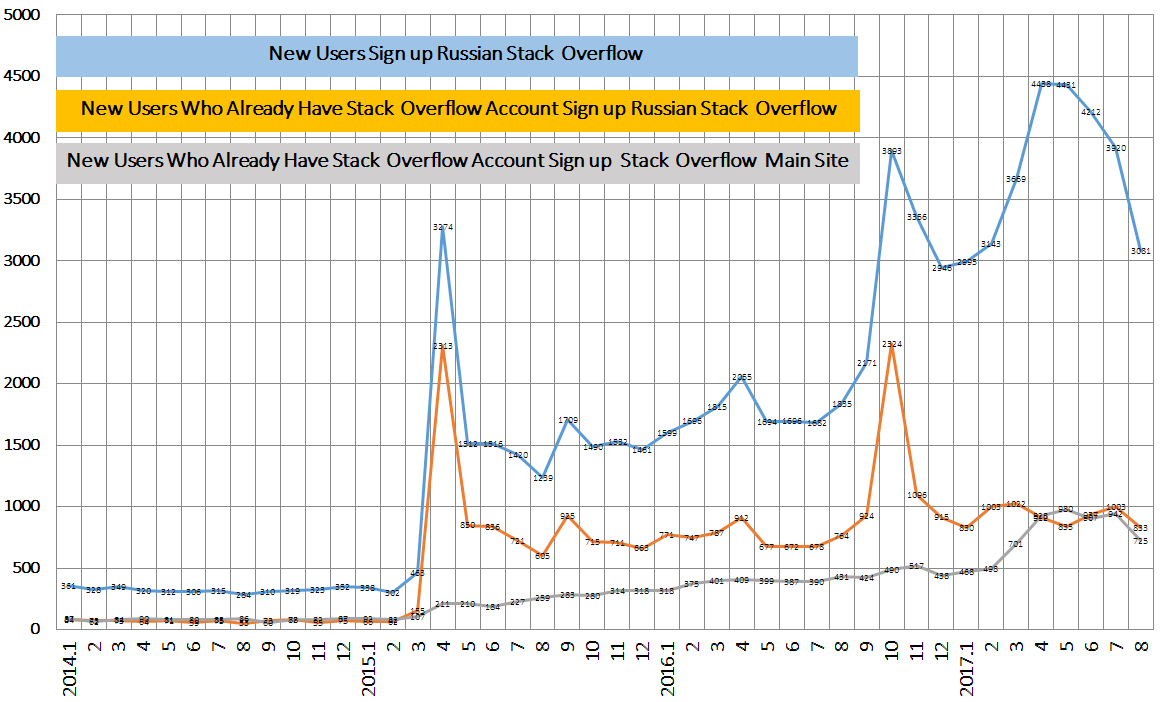
\includegraphics[width = 0.80\textwidth]{figures/userflow.png}
	\caption{New User Sign Up for Russian Stack Overflow}
\end{figure}
\subsection{Reputation}
Reputation is a mark [5], which represents how much contribution a user has made, how much the community trusts you and how much the peer users think about your work. Of course, the more reputation a user earned, the higher level of activity the user is. So it is very easy to measure the high-level user activity by calculating this variable. Figure 2.3 shows the statics of reputation of users in Russian Stack Overflow by segregating all 86,826 users into 3 groups. 
\par
Local users who do not own an account of the main site are 41,062, and the other two labels have been introduced are 29,609 and 16,155. The compare of user amount of these three groups shows in Figure 2.2.\par
\begin{figure}[h]
	%\centering
	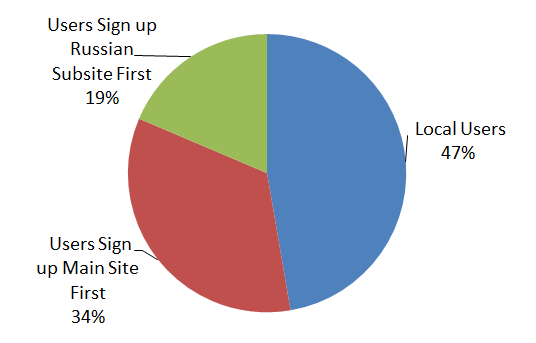
\includegraphics[width = 0.80\textwidth]{figures/pie.png}
	\caption{User Amount Compare for Russian Stack Overflow Users}
\end{figure}
Considering the Reputation Bonus Policy that a starting plus 100 reputation bonus to users who already have a 200+ account of any site belongs to Stack Exchange [5], the 29,609 users who migrated from the main site reasonably have a large number of the reputation level of 100 to 200. However, despite the local user, the remains are the user who owns both account of the main site and Russian version. Under the circumstance that the number of migrants is almost 2 times of that of the 16,155 users who sign up Russian version account first, the later contributes somehow an equal number of active users. \par
\begin{figure}[!h]
	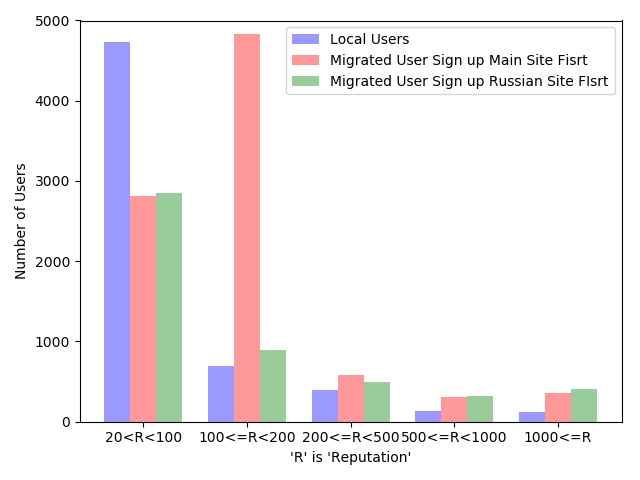
\includegraphics[width = 0.80\textwidth]{figures/reputation.png}
	\caption{Statics of Reputation}
\end{figure}
To some degree, the reputation reveals that multilingual communities are not dominated by a large number of external users even the later has an overwhelming advantage on the user amount, which means that multilingual communities are relatively independent in the respect of user contribution in the community development process.


\section{Post}
Although every user has the right to post a question and add comments, the composition of the knowledge base ought to obey the Pareto Law, which means 20\% of the users make 80\% of the contribution. In this section, we analyse the behaviours of those 20\% users. \par

Imagine that a post is a single unit, and millions of posts consist of the knowledge base, and each post includes maybe a lot of answers and comments in the tree structure. From Table 1 we know that there are totally 366,485 posts for the Russian Stack Overflow, and using the unique account id to calculate the amount of post for each user on Russian Stack Overflow, we have the results that present in Table 2.1. 

\begin{table}[!h]
	\centering
	\caption{Post Statics}
	\label{tab:table2}
	\begin{tabular}{|p{2.2cm}|p{2.0cm}|p{2.0cm}|p{2.0cm}|p{2.0cm}|}
		User Post count & Post Sum &Post Sum/ Post Amount& User Sum &User Sum/User Amount \\
		\hline
		P\_C$>=$2 &340,903&93.4\%&33,669&26.1\%\\
		P\_C$>=$4 &316,768&86.8\%&12,305&14.2\%\\
		P\_C$>=$6 &301,225&82.5\%&8,784&10.1\%\\
		P\_C$>=$8 &289,100&79.2\%&6,901&7.9\%\\
		P\_C$>=$10&278,688&76.4\%&5,665&6.5\%\\
	\end{tabular}
\end{table}	

\par
From the table, we can easily know the static distribution. As mentioned above, with the number of a single user post sum growing, the user proportion decrease. Notice that 5,665 people from the 86,826 Russian Stack Overflow users who have 10 or more posts contribute 76.4\% of the post amount. Here we need to set a research object called \'Core User\'. We need to assume these 5,665 people are the core users who have the highest level of contribution. Again, in these 5,665 core users, 1,685 people are local users while 3,980 people own both main site account and Russian sub-site account at the same time. In these 3,980 users in the intersection, 1,676 people are migrants from the Stack Overflow main site. Next, we will compare the level of the contribution between the migrants and the others in the Core User group. The user composition is showed in Figure 2.4.\par

\begin{figure}[!h]
	\centering
	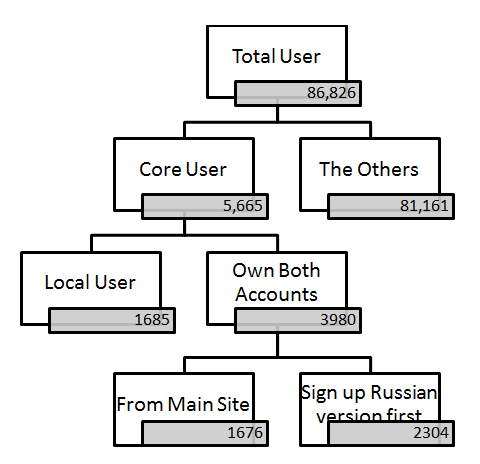
\includegraphics[width = 0.80\textwidth]{figures/usercomponent.png}
	\caption{Statics of components on Russian Stack Overflow}
\end{figure}
\par
For the 1,676 of Core Users who sign up the Stack Overflow account first, which also known as the migrant from the main site, they post 94,478 posts on Russian sub-site that count 25.9\% of the post amount on Russian sub-site. For the 2,304 of Core Users who sign up the Russian sub-site account first, which also known as the migrant from the main site, they post 125,891 posts on Russian sub-site that count 34.5\% of the post amount on Russian sub-site. According to the average level, the external users do not dominate the post area. 
\par
Moreover, for the 1,676 of Core Users who sign up the Stack Overflow account first, according to their frequency of post activity, we can also conclude that they are still spending more time and concentrate on the Stack Overflow main site. The formula of judging a migrant is Formula (2.1). If the f value is greater than 1, the user transferred his or her main active area to the new site.


\begin{normalsize}

	\begin{equation}
	f = \frac{Russian_PostSumAfterMigration/TimeLengthAfterMigration}{  Mainsite_PostCountBeforeMigration /TimeLengthBeforeMigration}	 
	\end{equation}
\end{normalsize}
\par
Assume that a reasonable range for the unchanged active level that is 0.8 to 1.2 for f, the results in Table 2.2 reveal that more than half of those active users from the main site tend to be more active in a multilingual sub\-site. Although they are from another site, they make a lot of contribution and seem to be like using the new sub-site regularly. The conclusion of the research on post aspect is the multilingual community has a group of users as backbone so that the community is not dominated by the users from the Stack Overflow main site, but the migrants from the main site are also willing to contribute in the new community.
\begin{table}[!h]
	\centering
	\caption{Statics for the 1,676 Users who post more than 10 and from Stack Overflow main site}
	\label{tab:table3}
	\begin{tabular}{|p{2.1cm}|p{2.2cm}|p{2.2cm}|p{2.2cm}|p{2.2cm}|}
		User Post count & User Amount & f $<$ 0.8 & 0.8$<=$f$<=$1.2 &f $>$ 1.2 \\
		\hline
		P\_C$>=$10 & 1,676  &637 & 106 & 933   \\
		P\_C$>=$20 & 400  & 187 & 35 & 178\\
		P\_C$>=$50 & 207 & 123 & 15 & 69 \\
		P\_C$>=$100& 132 & 93 & 10 & 29 \\
	\end{tabular}
\end{table}	

\section{Content}

\subsection{Tag}
A tag is a word or phrase that describes the topic of the question. The tag is a means of connecting experts with questions, and they will be able to answer the question by sorting questions into specific and well-designed categories. Research on the tags is able to reveal a number of most hot fields. There are 50,000 tags on Stack Overflow main site and 3,779 tags including 688 Russian character tags and 3091 non-Russian character tags on Russian sub-site. Ranking the top 10 frequent tags in several sets to show what are the most popular fields in both sites.
\par

\begin{table}[!h]
	\centering
	\caption{Tag Ranking Statics}
	\label{tab:table4}
	\begin{tabular}{|p{2.0cm}|p{1.6cm}|p{1.6cm}|p{1.6cm}|p{3.0cm}|p{3.0cm}|p{1.6cm}|}
		\hline
		Main site tags & f & Russian site tags & f & Russian site Russian tags &  Translation&f \\
		\hline
		javascript &0.339\permil & php &0.651\permil  & \foreignlanguage{russian}{массивы} &arrays  &0.066\permil \\
		\hline
		java &0.304\permil & javascript&0.583\permil  &\foreignlanguage{russian}{база-данных} &database & 0.062\permil\\
		\hline
		c\# &0.263\permil & java &0.531\permil  &\foreignlanguage{russian}{регулярные-выражения} & regular expressions&0.056\permil\\
		\hline
		php &0.259\permil & android &0.443\permil  &\foreignlanguage{russian}{алгоритм} &algorithm &0.056\permil \\
		\hline    
		android &0.238\permil & c\#&0.389\permil  &\foreignlanguage{russian}{веб-программирование} & web programming&0.042\permil\\
		\hline    
		jquery &0.201\permil & html &0.321\permil  & \foreignlanguage{russian}{вёрстка}&coding  &0.035\permil\\
		\hline    
		python &0.187\permil & jquery&0.282\permil  & \foreignlanguage{russian}{многопоточность}& multithreading & 0.030\permil\\
		\hline    
		html &0.159\permil & c++ &0.275\permil  &\foreignlanguage{russian}{ооп} &oop &0.028\permil\\
		\hline    
		c++ &0.123\permil & css &0.247\permil  &\foreignlanguage{russian}{строки} &lines&0.026\permil\\
		\hline    
		ios &0.122\permil & mysql &0.208\permil  & \foreignlanguage{russian}{файлы}&files&0.026\permil\\
		\hline 
	\end{tabular}
\end{table}	
According to the result shown in Table 2.3, it is clear that the popular areas of the two sites are similar. Considering the difference in the size of different communities, the hit counts of the same tag on different site are totally not on the same level. While for Russian Stack Overflow site, after translating the top 10 popular tags, it is clear that most of the Russian character tags are also common on the Stack Overflow main site. This fact indicates that for a series of website, all the tag sets of different language sub-sites are pretty similar, although there must be some distinction resulted by culture divergence.

\subsection{Links}
Link is a good tool to recommend and refer the existing works to other users. Not only links can refer the knowledge base in the same site, but also across different sites. This part of work is based on the statics of links on Stack Overflow main site and Russian Stack Overflow. People use links in their posts and comments, and connect their evidence and reference by links. The link amount and the direction reveal the similarity and difference between these two sites.
\par
Basically, in our study, links can be divided into two sets. One is the group of posts and comments refer the existing posts on Stack Overflow main site, and the other is those who refer the existing posts on Russian Stack Overflow. Some statistics are presented in the Table 2.4.
\begin{table}[!h]
	\caption{Links Statics}
	\centering
	\label{tab:table5}
	\begin{tabular}{|p{6cm}|p{3.5cm}|p{2.5cm}|p{2.5cm}|}
\hline
		 &Link Amount &Links referring posts of Stack Overflow&Links referring posts of Russian Stack Overflow\\
		\hline
		Stack Overflow Posts &13,187,126&1,512,118&80 \\
\hline	
		Stack Overflow Comments &5,737,401&1,759,284& 150\\
\hline		
		Russian Stack Overflow Posts &120,860&5,425&4,324 \\
\hline
		Russian Stack Overflow Comments &50,178&4,160&5,054 \\
\hline
	\end{tabular}

\end{table}	
\par
As we can see, the number of links that Russian users used to refer posts on Stack Overflow main site is smaller than the number of links that they used to refer posts on the Russian sub-site. Apparently, the results of the links show that Russian Stack Overflow sub-site is relatively independent because it owns a considerable proportion of links referring the existing post in its own knowledge base. The Russian sub-site does not completely depend on Stack Overflow main site, as the Russian users are not always referring the existing posts on main site. However, in some ways the Russian Stack Overflow sub-site has a non-negligible demand of knowledge reference from the main site. So the content of these two sites are not totally same and not totally different, especially the Russian subsite has its necessity of existence.

\section{Conclusion}
The above empirical comparison between two sites shows that Russian Stack Overflow owns many unique features which are not included by the main Stack Overflow, no matter its users or Russian-specific content.
Such difference demonstrate that the existence of the multi-lingual Stack Overflow is meaningful and useful to some specific users.
Furthermore, the multi-lingual deviation does not significantly undermine the knowledge accumulation or user participation of the main site.

Despite the uniqueness of the Russian site, there are a lot of interaction between two sites, e.g., many main-site posts are quoted in the Russian one.
In addition, as a relatively new site, questions asked in the Russian site may have already been posted in the main Stack Overflow site.
To assist site interaction and avoid potentially duplicated questions, a tool is needed to help retrieve related English posts in the main Stack Overflow when Russian users are asking or answering questions in the Russian site.

\begin{comment}
	Considering all the sections of analysis above, we can come to a solid conclusion that the multilingual community is meaningful not only according to the aspect of user activity but also the aspect of the knowledge base. Although the migration of users results in the change of user amount, the direction of the community development is still on a good track. Multilingual communities exist in form of different languages, but a large number of users are not limited in a single language. All the subsites and the Stack Overflow main site itself benefit from each other and form the positive relation.  \par
	
	
	However, there is one thing has been debated from the orientation day of the first multilingual community that how to solve the language gap and the segregation of knowledge base? If we can implement an approach that always recommends the valuable resources and overcome the language gap at the same time, the development of multilingual Q\&A community can be accelerated that every one of us can benefit from the breakthrough. \par
	
	
	So our approach is to utilize the current limit resource to generate satisfying results. Assume a foreign language speaker is using that language version of Stack Overflow subsite. Once he or she tries to find some helpful posts on the subsite, our approach can automatically utilize the tremendous knowledge base of the Stack Overflow main site to recommend the most k relevant posts. In this assumption, the data we can definitely receive includes a well-thought title and a list of tags that the user thought this question is related to. There is a well-developed corresponding system between posts and tags, also, according to the analysis of tags, they are sorted out in an efficient structure.
\end{comment}



%%% Local Variables: 
%%% mode: latex
%%% TeX-master: "thesis"
%%% End: 
